\documentclass[../main.tex]{subfiles}

\begin{document}


\section{Practical performance}
\label{section:analysis:pratic_performance}
\par In this section, we will look at the performance of our implementation. To do so, we developed a benchmark to showcase the performance of multiple scenarios. In each of these scenarios, we start with an empty filesystem to have a common base between all the situations. The benchmarks are run inside an Intel NUC running Ubuntu 18.04.4 with no particular intensive process already running. Furthermore, tests are run using the latest SGX SDK\footnote{SGX 2.9.1 at the time of writing.}. To avoid biased results, each test scenario is run up to 100 times.
\par During all the below scenarios, we will compare three filesystems: LAUXUS, the Linux ext4 and the \textit{FUSE} passthrough. This last filesystem just mirrors the usual filesystem (ext4). We chose to compare LAUXUS to ext4 to see the overhead incurred to the standard filesystem that most end-user is probably using. The comparison with the \textit{FUSE} passthrough was to see the impact of using \textit{FUSE}. The strange behaviour that we observed is that the \textit{FUSE} passthrough is more efficient than ext4 which is pretty particular but won't be discussed here as it is not the main concern of the work. We just want to compare LAUXUS performance compared to other filesystems.

\subsubsection{Copying operation overhead}
\label{section:analysis:write_overhead}
\begin{figure}[h]
    \centering
    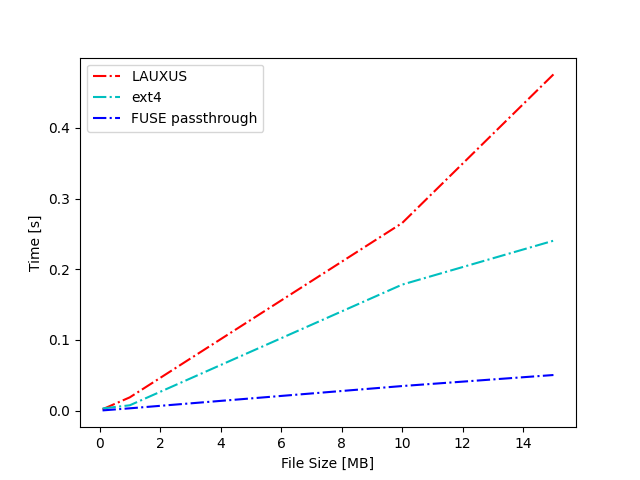
\includegraphics[width=.8\textwidth]{images/analysis/per_size}
    
    \caption{Copying time VS Size of the file}
    \label{figure:analysis:perf_write_per_size}
\end{figure}
\par In this experiment, we will look at the performance of writing a file into LAUXUS. This aims to see how our filesystem performs and deals with writing file of different sizes\footnote{we only checked the performance with the write operation because the read operation is similar and provides the same results}. Note that we are more interested in the evolution of the time instead of its absolute value. Indeed, having an exponential evolution is a huge limitation. From the design description, it is expected to have a linear evolution because, upon write, we only need to encrypt the edited block (which means it doesn't depend on the file size) and not the entire file.
\par As we can see from Figure \ref{figure:analysis:perf_write_per_size}, our implementation fits with our model because of the nearly linear evolution. Besides, we see that we have a sizeable overhead (two times slower than with ext4). Upon closer look, we see that the curve is not absolutely linear. This is because the size of the metadata structure increases throughout the copy operation. Further explanation of this behaviour is discussed in a subsequent section.

\subsubsection{Block writing time throughout an entire file write}
\begin{figure}[h]
    \centering
    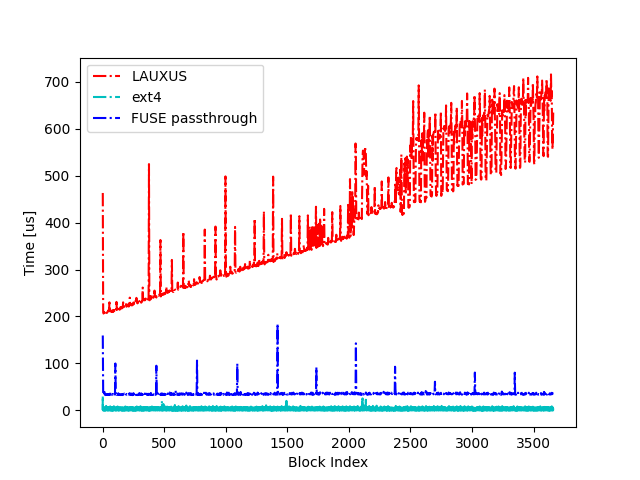
\includegraphics[width=\textwidth]{images/analysis/per_block}
    
    \caption{Evolution of the block writing time for a 15MB File}
    \label{figure:analysis:perf_time_per_block}
\end{figure}
\par In this experiment, we aim to see the evolution of the time it takes to write a block during a copy operation. We would expect from our model to take roughly the same amount of time to write each block during a copy operation.
\par As we can see from Figure \ref{figure:analysis:perf_time_per_block}, the write time is not constant throughout a full copy operation. This explains why we don't have a perfectly linear evolution in Figure \ref{figure:analysis:perf_write_per_size}. The reason for this behaviour is that on every write operation (write a single block), we are writing the entire metadata structure to the remote storage. We need to do so as we are creating a new content block and thus we must create a new block key. As the metadata structure becomes bigger and bigger, it takes more and more time to encrypt and write it. This is why we don't have a constant time.


\subsubsection{User entitlement overhead}
\label{section:analysis:user_entitlement_overhead}
\begin{figure}[h]
    \centering
    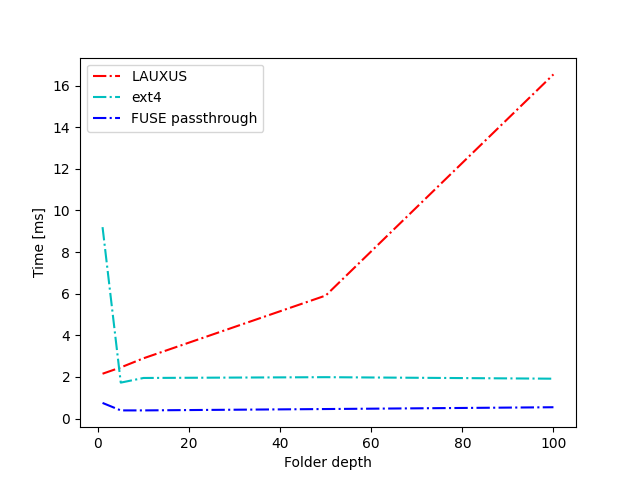
\includegraphics[width=.8\textwidth]{images/analysis/per_folder_depth}
    
    \caption{Copying time VS Depth of the file}
    \label{figure:analysis:perf_write_per_depth}
\end{figure}
\par This test is important because we have user entitlement on each directory level. Furthermore, because the names of the files are obfuscated, we must load the parent directories of the concerned file. Indeed, each Dirnode contains a mapping between each of its children name and their corresponding UUID. Furthermore, as there are multiple Dirnode level (with each a possibly different user entitlement), to de-obfuscate a file, we must load all of its parent directories.
\par This means that theoretically, the deepest in the hierarchy the file is (number of parent directories to the root), the more we need to check the user entitlement and load nodes, increasing the overhead on the access operation. Which means, we expect a linear evolution compared to the depth of the file. Fortunately, this process is done only one time: when the file is opened. Once open, the file structure stays in memory and we no longer need to check the hierarchy nor to load the parent directories to find the Filenode's UUID.
\par The Figure \ref{figure:analysis:perf_write_per_depth} illustrate the above theoretical explanation.
\par We see that this cause a considerable overhead when there are a lot of directories. However, increasing the delay to access a file of a few milliseconds is hardly noticeable to the end-users. As we are not aiming to use our filesystem in environments where extremely low latencies are required, we don't think that this requires further improvements.


\subsubsection{Writing a few bytes overhead}
\label{section:analysis:write_offset_overhead}
\begin{figure}[h]
    \centering
    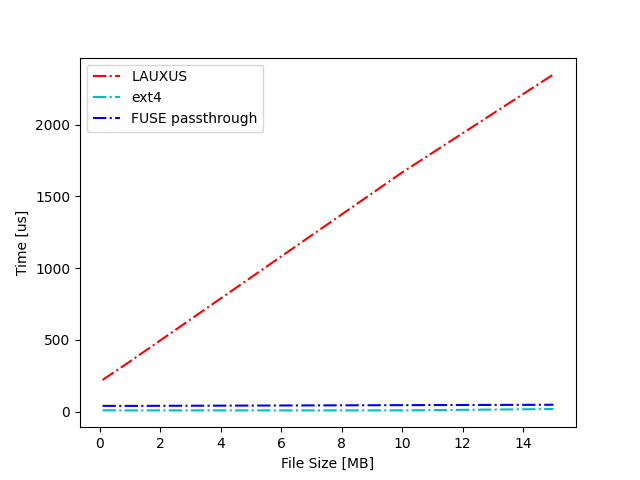
\includegraphics[width=.8\textwidth]{images/analysis/per_file_size_small_write}
    
    \caption{Writing a few bytes at different offset inside a 15MB file}
    \label{figure:analysis:perf_write_per_offset}
\end{figure}
\par The idea behind this test is to prove that if we need to make a small modification to a big file, it has the same performance as making the same modification to a way smaller file. Indeed, as our model is splitting a file into multiple blocks, when we edit a block, we just need to encrypt and save this precise block, not all the others. This means that we should expect no evolution when the file becomes bigger.
\par By inspecting Figure \ref{figure:analysis:perf_write_per_offset}, we may think that our implementation doesn't fit our model as our time evolves kind of linearly. It is not constant because we must first load the metadata of the filenode in memory. This simply means that the bigger the file is, the bigger the metadata is and thus the longer it takes. We can be pretty confident that this reasoning is correct because, between the smallest and biggest file (from 0.1 MB to 15 MB), it increases of only a few milliseconds.


\subsubsection{Block size impact on copy operation}
\label{section:analysis:block_size_impact}
\begin{figure}[h]
    \centering
    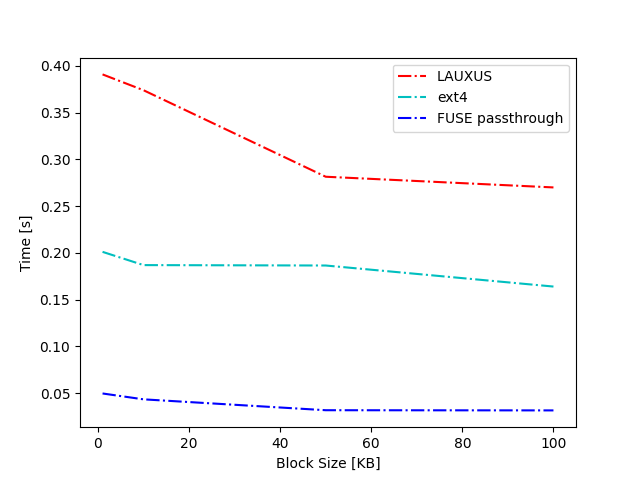
\includegraphics[width=.8\textwidth]{images/analysis/per_block_size}
    
    \caption{A 10MB File writing time VS block size}
    \label{figure:analysis:block_size_impact}
\end{figure}
\par Depending on each user-space application, the application may write their information with blocks of different sizes (e.g: nano makes write operations of maximum 1KB, vim makes write operations of maximum 2KB, etc). This test is to check how our implementation behaves in those cases. Having a non-constant time means that depending on the user-space application the end-user is using, it may result in different performances.
\par By inspecting Figure \ref{figure:analysis:block_size_impact}, we see that we are more efficient if we are writing blocks of larger sizes.
\par As our implementation is using a stateless model (no session) for writing the encrypted file to the remote storage, the more we increase the block size, the more we are efficient (to a certain threshold). By stateless model, we just mean that on each write operation, we open the file on the remote storage then apply the operation then we close the file. A more efficient approach would be to open the file at the same time the end-user opens it (with the open operation) and similarly when closing it. However, this should not highly change our performances as the writing time is mainly governed by the encryption time.


\subsubsection{Unzip folders}%zip size over 1.4M and zip content 3.2
\label{section:analysis:zip}
\begin{figure}[h]
    \centering
    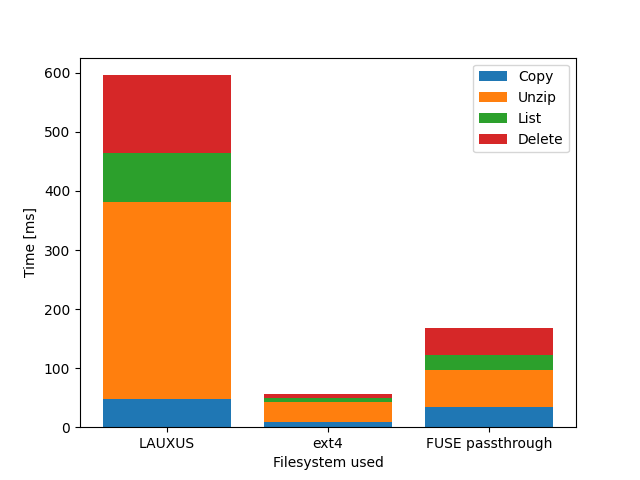
\includegraphics[width=.8\textwidth]{images/analysis/zip}
    
    \caption{Zip scenario}
    \label{figure:analysis:zip}
\end{figure}
\par This scenario is to showcase that LAUXUS can be used by other filesystem programs (zip in this case). The scenario is really simple, it consists of copying an archive inside LAUXUS, unzip it, list all the files in the unzipped folder\footnote{using the tree command} and lastly delete the entire unzipped folder. We chose this scenario as it regroups a lot of different operation that could be done in a real-life situation. The chosen archive is simply the LAUXUS repository. It has a size of $1.4$MB zipped and $3.2$MB unzipped.
\par As expected, LAUXUS is slower than both filesystem but in the end, the whole operation is still pretty fast and doesn't incur a noticeable overhead to the end-user.
\par Surprisingly by analysing the Figure \ref{figure:analysis:zip}, we see that ext4 becomes faster than the \textit{FUSE} passthrough which is the opposite than what we saw in the other scenarios. However, this seems logical as \textit{FUSE} can't be faster than ext4 because it just mirrors ext4. We suppose that the reason the other scenarios were at the advantage of \textit{FUSE} may come from a special operation in \textit{FUSE} to regroup operation together for efficiency.


\subsubsection{Memory and CPU usage}
\label{section:analysis:memory_cpu_usage}
\begin{figure}[h]
    \centering
    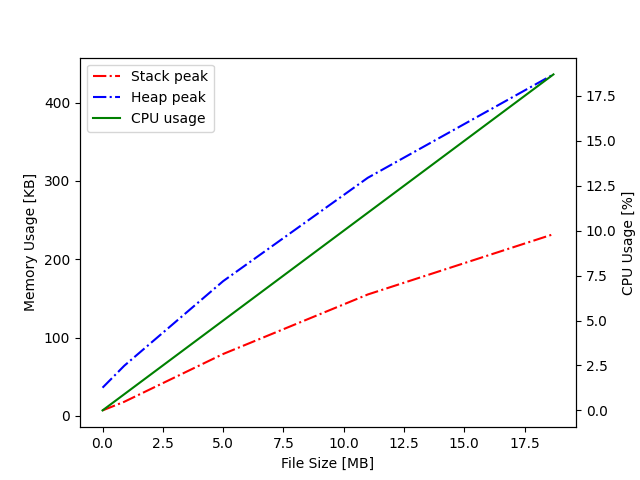
\includegraphics[width=.8\textwidth]{images/analysis/memory_cpu_usage}
    
    \caption{Memory and CPU usage when copying a single file}
    \label{figure:analysis:memory_cpu_usage}
\end{figure}
\par This last test is rather different than all the above ones. We don't compare to the other filesystem (ext4 and passthrough) because we are more interested in the absolute values and how they evolve. Furthermore, the memory usage is specific to the Enclave. Indeed, this measure represents the maximum amount of memory needed to execute the operation. The operation chosen here is just copying a single file like in Section \ref{section:analysis:write_overhead}.
\par By analysing the Figure \ref{figure:analysis:memory_cpu_usage}, we see that our software is quite demanding in memory space as discussed in Section \ref{section:analysis:limitations}. Indeed, as inside an Enclave, both the Stack and Heap size are limited, we can encounter issues when dealing with a very big file (e.g: 1GB). Solutions for this limitation are explained in \ref{section:analysis:limitations}.
\par The good news about all the curves is that they don't behave exponentially which is very promising for the software. This means that if the issues discussed in Section \ref{section:analysis:limitations} are solved, the application can be used without limitations (e.g: with very big files, etc).


\end{document}